\documentclass[a4paper, 12pt,oneside]{article} 
%\documentclass[a4paper, 12pt,oneside,draft]{article} 

\usepackage{preamble}
\usepackage{bm}

%--------------------- ACTUAL FILE ---------------------- %
\begin{document} 
	\begin{center}
	    \Large
	    \textbf{RL mini-project : Mountain Car environment}
	        
	    \vspace{0.4cm}
	    \large
	    Authors : Rayan Harfouche \& Tara \footnote[1]{My administrative name is Tobia, so you will find me under that name in EPFL related databases.} Fjellman \\
	    \small{Spring 2024}
	\end{center}

    \section{Introduction}
        To be written after the rest of the report is done.

    \section{Environment}
        The Mountain Car environment is a RL environment in which the agent is placed in a valley between two hills. The goal is for it to learn to reach the top of the right hill. The agent can only apply a force of -1, 0 or 1 to the car. The state space is continuous and has two dimensions, the position and the velocity of the car. The domain is [-1.2,0.6] for the position and [-0.07,0.07] for the speed. The agent receives a reward of -1 at each time step, and a reward of 0 when it reaches the top of the hill. The episode ends when the agent reaches the top of the hill or after 200 steps. 
    \section{Random agent}
    \begin{wrapfigure}{r}{0.5\textwidth}
        \centering
        \vspace{-3em}
        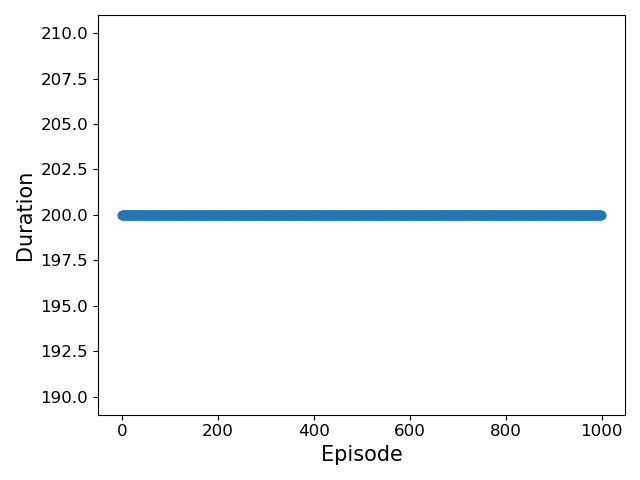
\includegraphics[width=0.5\textwidth]{../runs/random/n_eps=1000/figs/duration}
        \caption{Episode duration of random agent during training.}
        \label{fig:random-neps=1000}
    \end{wrapfigure}
    We start by running a random agent, i.e. one that selects its action at random. To analyse its performance, we inspect the duration of the episodes. Indeed, if the agent solves the task, the duration of the episodes should be lower than 200\footnote[2]{... of course except if it solves the task in exactly 200 steps.} (as this is the truncation time).
    Running the the agent for 1000 episodes, we obtain \ref{fig:random-neps=1000}. Looking at it, it is clear that the agent does not succeed at the task. Actually the agent just oscillates around the minimum.
    \section{DQN}
    We now turn to the DQN agent. Now the policy is actually learned and should lead to better results. 
        \subsection{Vanilla version}
        Running 1000 episodes and computing : the duration of the episodes along with the episode-cumulated reward and loss, we get \ref{fig:dqn-vanilla-neps=1000}. Looking at it we see that the behaviour is the same as for the random agent, i.e. the agent does not learn the task. This is due to the sparsity of the reward. Indeed, without reward, the agent does have information to adapt. 
        \begin{figure}[h!]
            \centering
            \vspace{0em}
            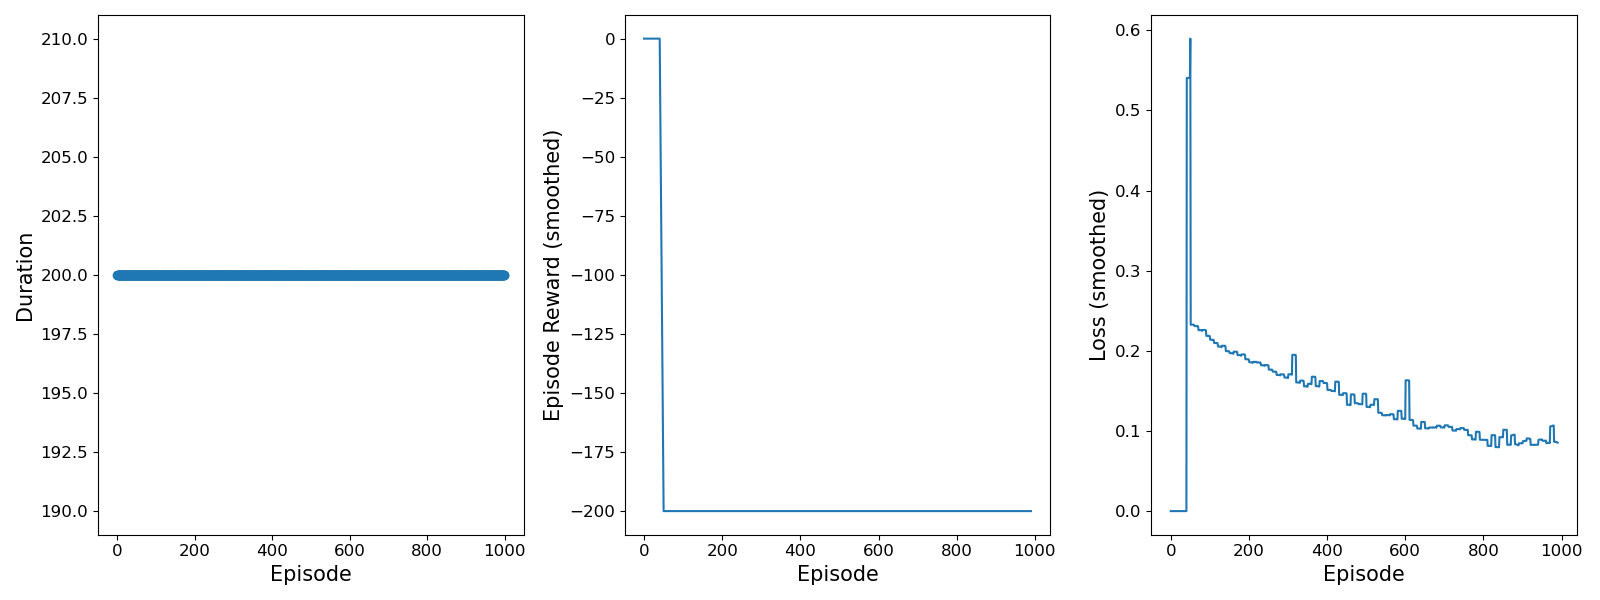
\includegraphics[width=.9\textwidth]{../runs/dqn_vanilla/up-tau=1/figs/full_results}
            \caption{Results associated to the training of a vanilla DQN agent.}
            \label{fig:dqn-vanilla-neps=1000}
        \end{figure}
        %\subsection{Training metrics}
        %To analyse further the training behaviour of our agents we can look at the loss and reward per episode. We can moreover look at the cumulative (cumulated) reward and cumulative successes over the episodes. $
        
        \subsection{Auxiliary reward}
        To help the agent learn, we now introduce auxiliary rewards that will be added to the environment reward. Theses should promote exploration, contering the sparsity of the reward. 
        \subsubsection{Heuristic reward}
        \subsubsection{Chosing the function}
        \begin{wrapfigure}{r}{0.5\textwidth}
            \centering
            \vspace{-1em}
            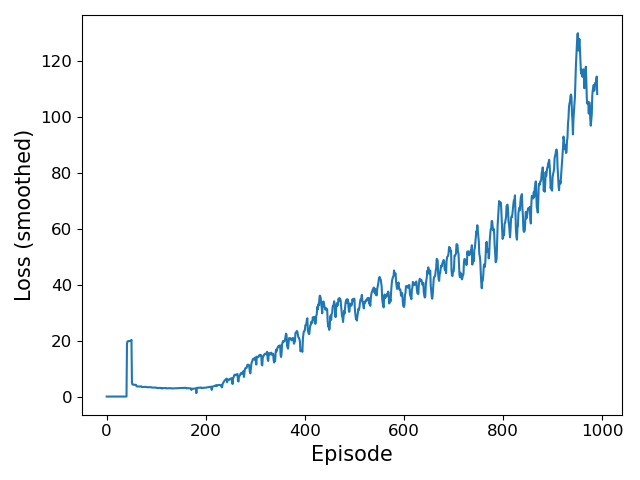
\includegraphics[width=0.5\textwidth]{../runs/dqn_heuristic/up-tau=3_d=2_frac=3.5/figs/loss}
            \caption{Evolution of cumulative training loss as a function of the episode for a heuristic reward agent. The reward factor is set to 3.5 and the loss is smoothed with a window of width 10.}
            \label{fig:dqn-heuristic-frac=3.5-loss}
        \end{wrapfigure}
        Intuitively, we want this function reward the agent when it makes an effort to reach the top of the hill. We therefore decide to take a heuristic function that is monotonous in the height of the mountain car. The (normalised) height can be deduced from the position as
        $$
        h(x) = \frac{1-\cos\left(\frac{x-x_0}{x_r-x_0}\pi\right)}{2},
        $$
        where $x_0$ and $x_r$ respectively are the average-starting and ending positions. 
        A simple and versatile reward function is therefore  
        $$
        f(x) = Ah(x)^n - A
        $$
        for $A\ge 0$ some constant we call reward-factor and a given $n\in\mathbb N^\star$. The $-A$ offset is there to make extra sure that for all values of the scale factor $A$, the agent does not get tempted to stay and collect the heuristic reward, we decide to offset the function by its maximal value (i.e. $A$). This way, the heuristic reward is always negative, and the agent is encouraged to reach the top of the hill.
        To check that this version of the agent is learning, we plot (for $A=...$) the loss (see \ref{fig:dqn-heuristic-frac=3.5-loss}), the duration (see \ref{fig:dqn-heuristic-frac=3.5-duration}) and the collected reward (see \ref{fig:dqn-heuristic-frac=3.5-reward}) during learning. Looking first at \ref{fig:dqn-heuristic-frac=3.5-duration}, we see that the agent solves the task in less than ... episodes. Now turning to \ref{fig:dqn-heuristic-frac=3.5-reward}, it is interesting to notice that during the time the agent fails at the task (for episodes $\le 250$) the auxiliary reward increases. This means that the agent is exploring heigher and heigher states. After some time, it actually reaches the top of the hill, and so learns that it can increase its environement reward by doing so. This is exactly what we wanted to achieve with the heuristic reward !
        As for the loss, we see that it is increasing, which might come to a surprise. Indeed in machine learning we are used to seeing training lossess decrease. In this case however, the loss is just an indicator of how well the agent is learning the Q function. The observed increase actually corresponds to the fact that the learning of this function gets harder as its domain increases.
        \begin{figure}[h!]
            \centering
            \vspace{0em}
            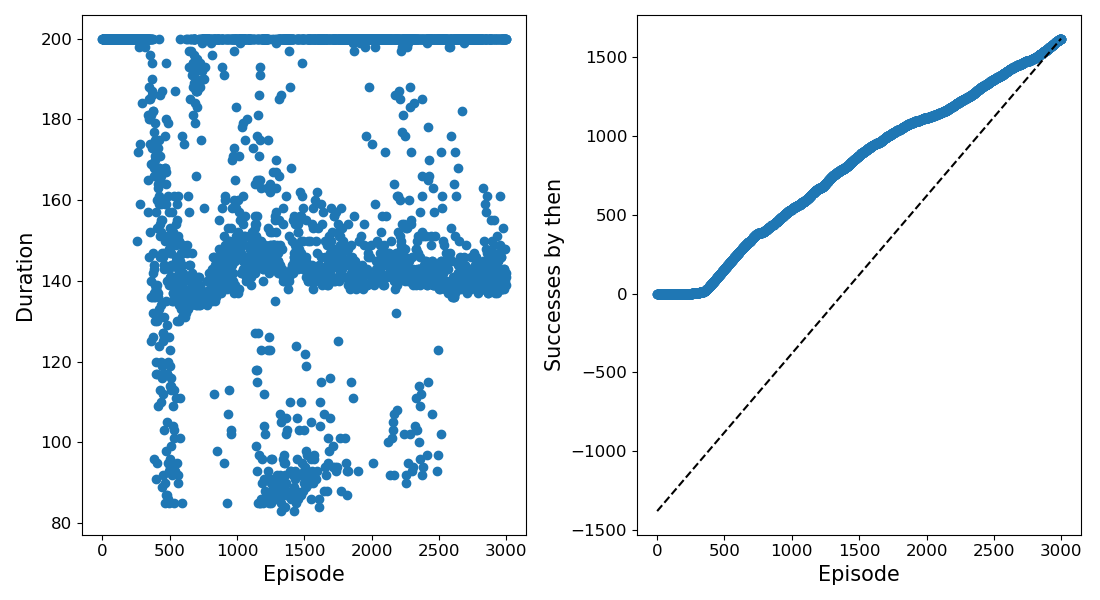
\includegraphics[width=.75\textwidth]{../runs/dqn_heuristic/up-tau=3_d=2_frac=3.5/figs/duration}
            \caption{Evolution of episode duration and cumulative number of successes as a function of the episode for a heuristic reward agent. The reward factor is set to 3.5.}
            \label{fig:dqn-heuristic-frac=3.5-duration}
        \end{figure}
        \begin{figure}[h!]
            \centering
            \vspace{0em}
            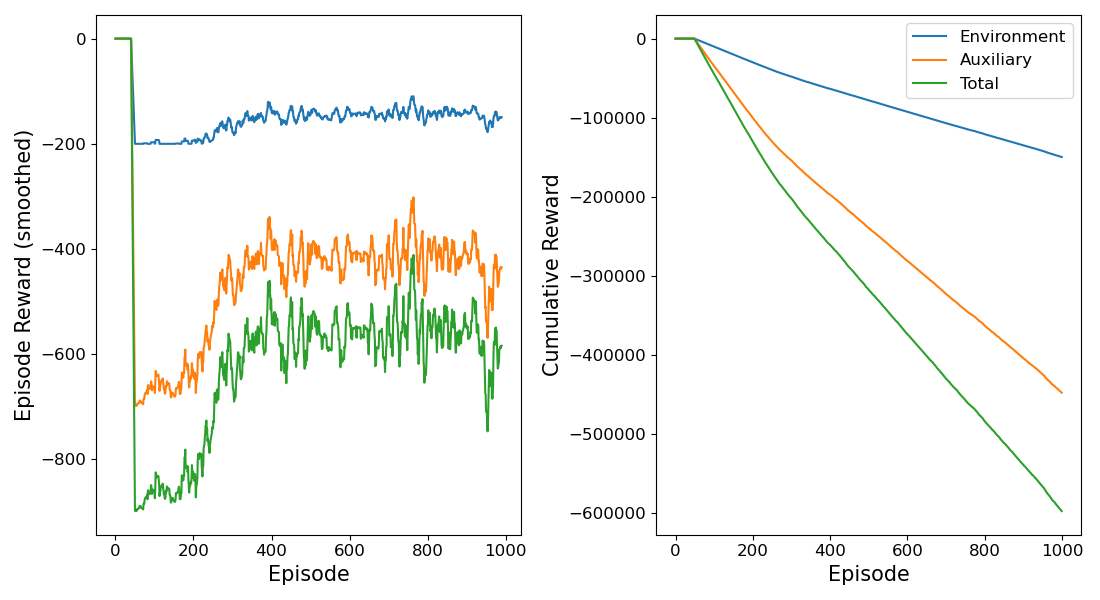
\includegraphics[width=.75\textwidth]{../runs/dqn_heuristic/up-tau=3_d=2_frac=3.5/figs/reward}
            \caption{Evolution of cumulative reward and cumulated cumulative reward (over the different episodes) as a function of the episode for a heuristic reward agent. The reward factor is set to 3.5 and the cumulative reward is smoothed with a window of width 10.}
            \label{fig:dqn-heuristic-frac=3.5-reward}
        \end{figure}
        \subsubsection{Auxiliary reward scaling}
        For the auxiliary reward to be useful, it should intuitively not be too small. Otherwise the situation would be no different than for the vanilla agent. As for the upper bound, we impose that it should not dominate the environment reward. Indeed, otherwise the agent could learn to collect the reward during the full 200 steps instead of reaching the goal. The exact value of this upper bound is not easy to express analytically, but we expect it to be of order 1. This provides us with a crude guess, which we can refine by testing different values.
        \begin{figure}[h!]
            \centering
            \vspace{0em}
            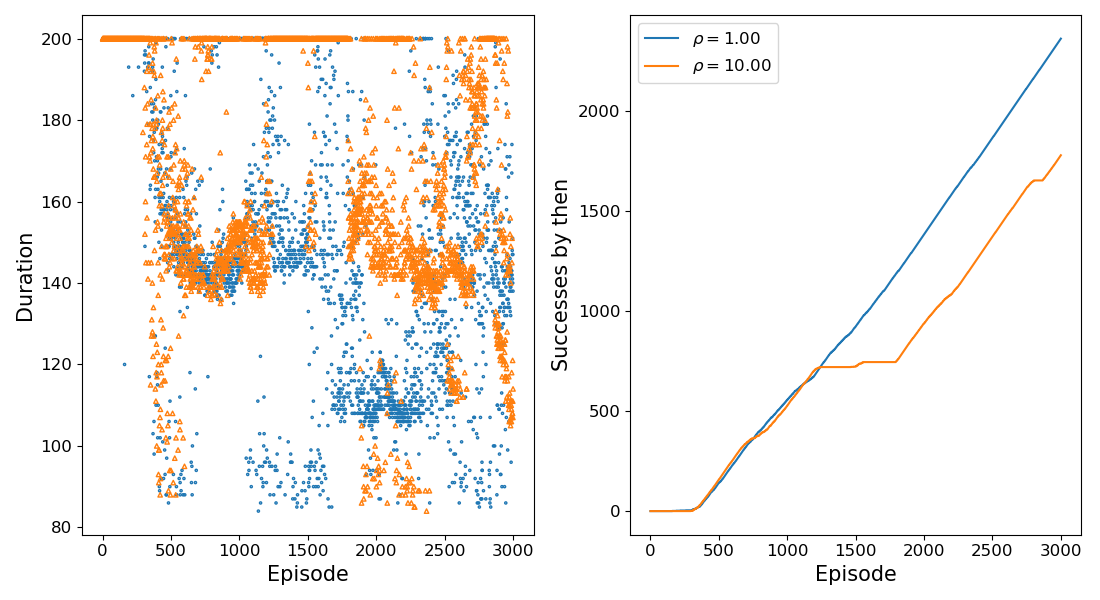
\includegraphics[width=.75\textwidth]{../runs/dqn_heuristic/comparison}
            \caption{Evolution of episode duration and cumulative number of successes as a function of the episode for a heuristic reward agent. The different colours correspond to different values of the reward factor}
            \label{fig:dqn-heuristic-comparison}
        \end{figure}
        To analyse the effect of the reward factor on the performance, the heuristic agent was run for multiple valuees of the parameter. The corresponding results are shown in \ref{fig:dqn-heuristic-comparison}. We see that ...
        %the agent is able to solve the task for all values of the reward factor. 
        %However, the time it takes to do so varies. This is expected, as the reward factor is a scaling parameter. The larger it is, the more the agent is encouraged to explore. This is why the agent is able to solve the task for all values of the reward factor.
            %* test the higher reward with low degree func ? 
            %* be on the lookout for instabilities 
        %Indeed, one could think that the optimal strategy would be to go right->left->right with as large swings as possible. However, doing so results in an unnecessary large (and time-consuming) left swing, since as seen in the first solution the first (non large) swing is sufficient to obtained the necessary speed. The 
        \section{RND reward}
        In this section we consider the results associated to the RND auxiliary reward agent.
            \subsection{Normalisation} 
            As recommended by the hint, we standardise the input and output of the RND network. The input standardisation is done since we want the output to vary as a function of how different the observed state is compared to the previously visited ones. Indeed, subtracting the typical state (i.e. the mean one) provides a good idea of how different the new input state is. The normalising by the typical distance from the mean state (i.e. the standard deviation) is done to make sure the input is of order 1, which is a good practice for neural networks to avoid instabilities.
            
            The standardisation of the output is instead done to control the characteristics of the RND reward attributed to the states. Indeed, by subtracting the mean we make sure that typical states are penalised  while new ones are rewarded; while normalisation makes it possible to tweak the the order of magnitude of the reward. The clamping is done for this same last reason (as NNs can produce a heavy tail output). 
            % but then why not the in Q net ? can't scale the environment to gain stability ?
            \subsection{Reward-factor scale}
            \begin{wrapfigure}{r}{0.5\textwidth}
                \centering
                \vspace{-1em}
                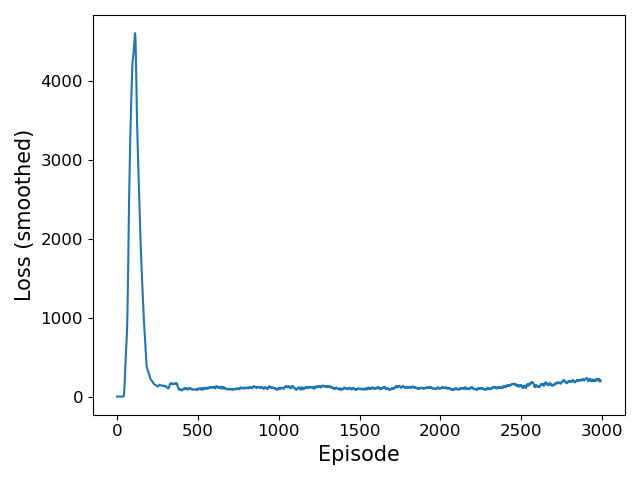
\includegraphics[width=0.5\textwidth]{../runs/dqn_rnd/up-tau=1_r-fact=35.0/figs/loss}
                \caption{Evolution of cumulative training loss as a function of the episode for a RND reward agent. The reward factor is set to 3.5 and the loss is smoothed with a window of width 10.}
                \label{fig:dqn-rnd-r-fact=35-loss}
            \end{wrapfigure}
            Mostly the same argument applies as for the heuristic reward. This time however, if the factor is taken too large, we expect the agent to prefer exploring instead of ending the episode by reaching the top of the hill. Indeed, when the agent will have reached the top of the hill a few times, the states that will have allowed it to do so will have a low RND reward. This is because the RND network will have seen them many times, and so the prediction error will be low.
            * crude scale : over an episode the rewards should be comparable ?? 
          \begin{figure}[h!]
            \centering
            \vspace{0em}
            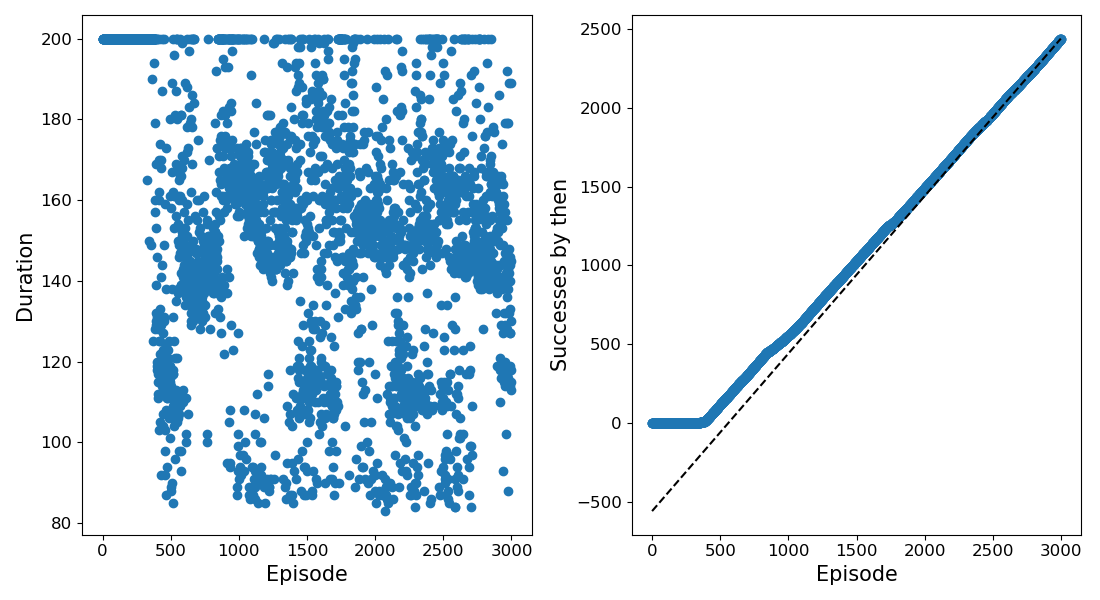
\includegraphics[width=.75\textwidth]{../runs/dqn_rnd/up-tau=1_r-fact=35.0/figs/duration}
            \caption{Evolution of episode duration and cumulative number of successes as a function of the episode for a heuristic reward agent. The reward factor is set to 3.5.}
            \label{fig:dqn-rnd-r-fact=35-duration}
        \end{figure}
        \begin{figure}[h!]
            \centering
            \vspace{0em}
            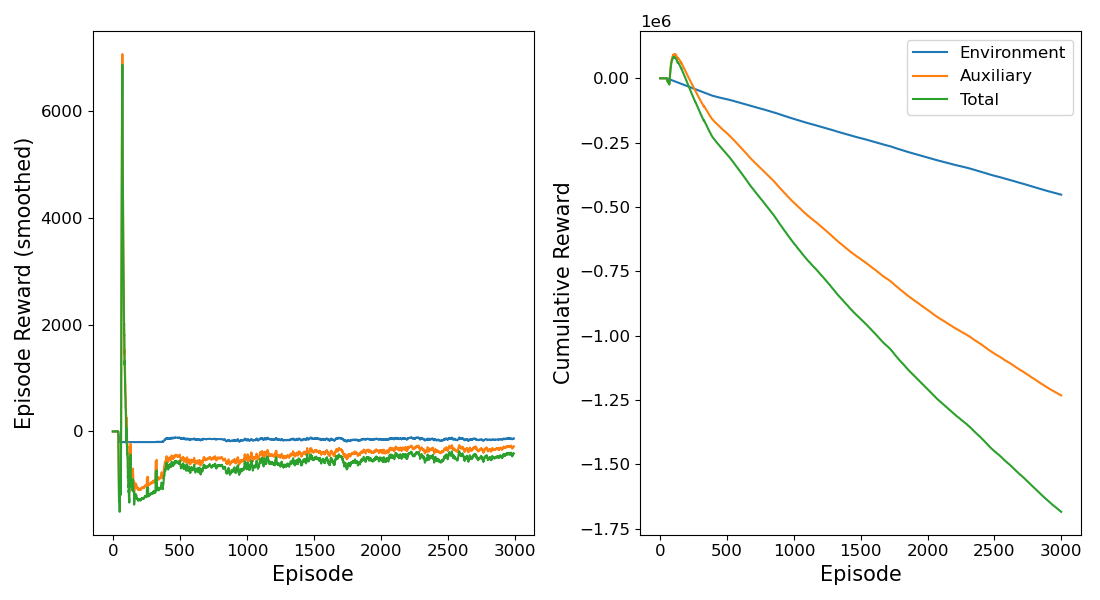
\includegraphics[width=.75\textwidth]{../runs/dqn_rnd/up-tau=1_r-fact=35.0/figs/reward}
            \caption{Evolution of cumulative reward and cumulated cumulative reward (over the different episodes) as a function of the episode for a heuristic reward agent. The reward factor is set to 3.5 and the cumulative reward is smoothed with a window of width 10.}
            \label{fig:dqn-rnd-r-fact=35-reward}
        \end{figure}
        \subsection{Comparison to heuristic reward}
        * difference in behaviour : we oscillate between the two possible solutions. This can be explained by the fact that the RND reward penalises the agent for repeating moves, and therefore leads the agent to switch its method more. 
    \section{Dyna}
        The Dyna algorithm relies on the discretization of the phase space (space of positions and velocities).
        The main parameter that will be varied in this section is this section is the size factor $\alpha$. We take as a reference of the step sizes the vector suggested in the project description ($\Delta x_0, \Delta v_0$) = (0.025, 0.005). We then test discretizations of the form ($\Delta x, \Delta v$) = $\alpha$ ($\Delta x_0, \Delta v_0$) 
        for different values of $\alpha$.

        \subsection{Dyna manages to solve the task!}
        When considering the original discrtization ($\alpha=1$), we observe that the task is solved, in the sense that successes (defined by episodes where the target is reached before 200 steps) are observed. 
        As in the previous sections, we plot the duration of each episode during the training, as well as the number of success with respect to the number of episodes. 
        In Figure \ref{dyna_first}, we show the result for $\alpha=1.5$ considered as a value allowing a good training (better than $\alpha=1$). We also plot results for values $\alpha=0.55$ and $\alpha=4.5$. 
        
        \begin{figure}[h]
            \centering
            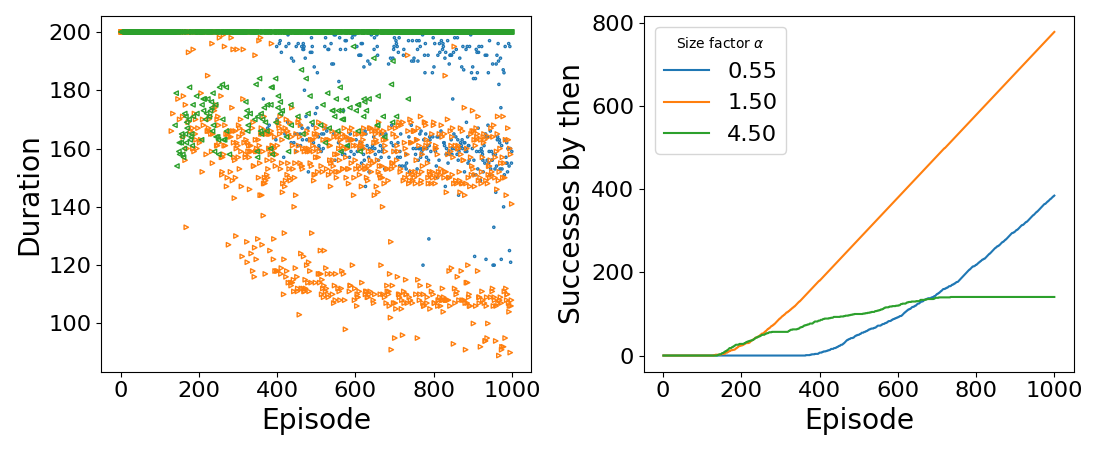
\includegraphics[width=0.9\textwidth]{../runs/dyna/dyna_comparison.png}
            \caption{}
            \label{dyna-first}
        \end{figure}
        
        Value $\alpha=1.5$ shows a good performance as first successes are observed before 200 epsiodes. Then the line of success becomes wrt to the number of epsiodes becomes a line of slope 1. 


        
        \section{Comparison of the agents}
        In this section we compare heuristic and RND DQN agents to the Dyna agent. 
        
        We first do so for the training phase by training each of these agents for 3000 episodes, and then plotting their associated enverionement reward evolution. The results are shown in ref{...}.
        %
        We can see that ....

        Now we compare the performances by running each of the trained agents for 1000 additional episodes in `evalutation mode', i.e. using a greedy policy. The plots of the corresponding episode durations are shown in ref{...}. To reduce stochastic fluctuations the results are made on the same environement seeds across the agents.
        \begin{figure}[h!]
            \centering
            \vspace{0em}
            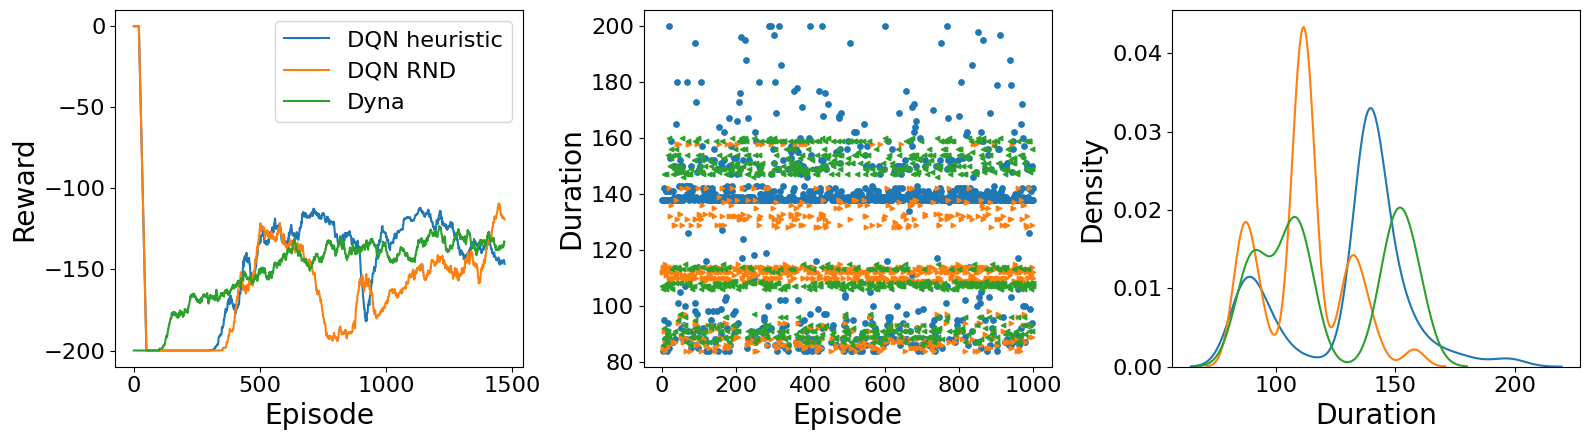
\includegraphics[width=.75\textwidth]{../code/comparison}
            \caption{Episode durations of heuristic and RND DQN agents and Dyna agent.}
            \label{fig:agent-performance-comparison}
        \end{figure}
        %
        We can see that ....
        \section{Conclusion}
        \subsection{Two types of solutions ?}
        From the plot of the episode durations, we can see that the agent seems to have two distinct behaviours. Indeed, we can see that the density of points is larger for $90<d<120$ and $150<d<180$ than in between of these ranges. Investigating this more closely (inspecting the trajectories associated to these performances), one can trace this difference back to the initial condition. 
        
        If we start on the right of the minimum, we are able to reach the goal fast by only 2 large swings : the first to the left and the second to the right. If we start on the left of the minimum, the solution takes longer. Indeed, we need to go right, then left, then right again. This is due to the fact that the car has to gain enough speed to reach the top of the hill.
        Notice that the distinction between these two solutions is not that sharp. This is due to the fact that the initial condition is uniform over $[-0.6,-0.4]$, and so the agent sometimes starts close to the minimum, and therefore is not exactly in any of the two cases. 
        \section{Appendix}
\end{document}